\section{Empirical Validation}
\label{sec:exp}

To demonstrate the practical value of the theory developed in the previous
sections, we argue that our techniques
\begin{itemize}

  \item scale far beyond existing algorithms, and

  \item are complete in practice.

\end{itemize}
To argue these points we have implemented three basic refinement-checking
algorithms.

\begin{description}

  \item[{\sc enumerate}] is our implementation of the classical
  linearizability-checking algorithm~\cite{journals/jpdc/WingG93} implemented
  by Line-up~\cite{conf/pldi/BurckhardtDMT10}, checking each history $h$ by
  enumerating the linearizations $h'$ of $h$'s completions. We check whether
  each $h'$ is included in the kernel $H$ by asking\footnote{Classically this
  check is performed by set inclusion, as the length of $h$ is assumed to be
  bounded by some number $n \in \mathbb{N}$ of operations, and the subset $H_n
  \subseteq H$ of $n$-operation histories of $H$ is computable in finite time.
  As we assume no such bound on the number of operations, we perform this check
  via theorem-prover query instead.} whether $h' \models \textsc{Theory}(H)$.
  As soon as this check succeeds, we conclude that $h \in \overline{H}$.
  Otherwise if this check fails for all linearizations, we conclude $h
  \not\in \overline{H}$.

  \item[{\sc symbolic}] checks each history $h$ by reduction to the
  satisfiability of $\textsc{Stronger}(h) \land \textsc{Theory}(H)$, as
  described in Section~\ref{sec:propositional}, delegating the enumeration of
  both completions and linearizations to an underlying solver. If the
  satisfiability check succeeds, or is inconclusive, we conclude that $h \in
  \overline{H}$. Otherwise if unsatisfiability is found, we conclude that $h
  \not\in \overline{H}$.

  \item[{\sc saturate}] avoids the expensive propositional backtracking
  inherent to the aforementioned {\sc symbolic} checker by limiting the
  satisfiability check to Boolean constraint propagation. Essentially, we
  implement a customized incremental solver which only saturates with unit
  propagation, avoiding any propositional branching. If a contradiction is
  found, we conclude that $h \not\in \overline{H}$. Otherwise if saturation
  fails to reveal a contradiction, we conclude $h \in \overline{H}$.

\end{description}
Additionally, we have implemented the removal of obsolete matches as outlined
in Section~\ref{sec:obsolete}, which can be enabled for the {\sc symbolic}
and {\sc saturate} algorithms.

We have studied ten concurrent data structure implementations from the
Scal\footnote{\url{http://scal.cs.uni-salzburg.at}} High-Performance
Multicore-Scalable Computing suite. Six of these implementations, such as the
Michael-Scott Queue~\cite{conf/podc/MichaelS96}, are meant to preserve
observational refinement\footnote{More precisely, they are designed to be
linearizable.} while the other four, such as the non-blocking
bounded-reordering queue~\cite{conf/pact/KirschLP13}, are meant to preserve
weaker properties.

The input to our checking algorithms are histories given as text files
consisting of line-separated call and return actions. For the selected set of
concurrent object implementations, we generated the histories of several
executions under pseudo-random scheduling by logging calls and returns in the
order in which they occurred. While scanning an input history, the selected
algorithm performs a membership test at each prefix at which an operation
completes --- i.e.,~at return actions.

Our first set of experiments (\S\ref{sec:exp:scalable}) demonstrates that our
symbolic algorithms are drastically more scalable than existing algorithms, in
that they are able to process vastly more history operations in much shorter
time. Our second set of experiments (\S\ref{sec:exp:complete}) demonstrates
that our more efficient algorithms are complete in practice: the violations
surfacing in the logs of actual executions are consistently discovered. We made
all measurements on similar MacBook Pro 2.XGHz Intel Core i5/i7 machines, and
discharged theorem-prover queries with an in-process instance of
Z3\footnote{\url{https://github.com/Z3Prover/z3}}.

Our implementation of the algorithms and all (generated) histories used in
these experiments, are available on
GitHub\footnote{\url{https://github.com/imdea-software/observational-refinement-checking}}.

\subsection{Scalability of Symbolic Checking}
\label{sec:exp:scalable}

Our first experiment measures the number of steps each algorithm is able to
process for varying time limits over $10$ histories of Scal’s Michael-Scott
Queue implementation with $10000$ steps each. We used five per-history time
limits of $5$s, $25$s, $50$s, $75$s, and $100$s. Results are shown in the graph
of Figure~\ref{fig:steps} — results are similar for the other nine Scal
implementations. The {\sc enumerate} algorithm performs worst, progressing only
from median $18$ steps in $5$s to median $32$ steps in $100$s. The {\sc
symbolic} algorithm is a significant improvement, progressing from median $37$
steps in $5$s to median $70$ steps in $100$s. While adding match removal helps,
achieving roughly an order-of-magnitude improvement over {\sc enumerate}, the
cost of checking remains exponential in the number of steps.

\begin{figure}[t]

  \centering
  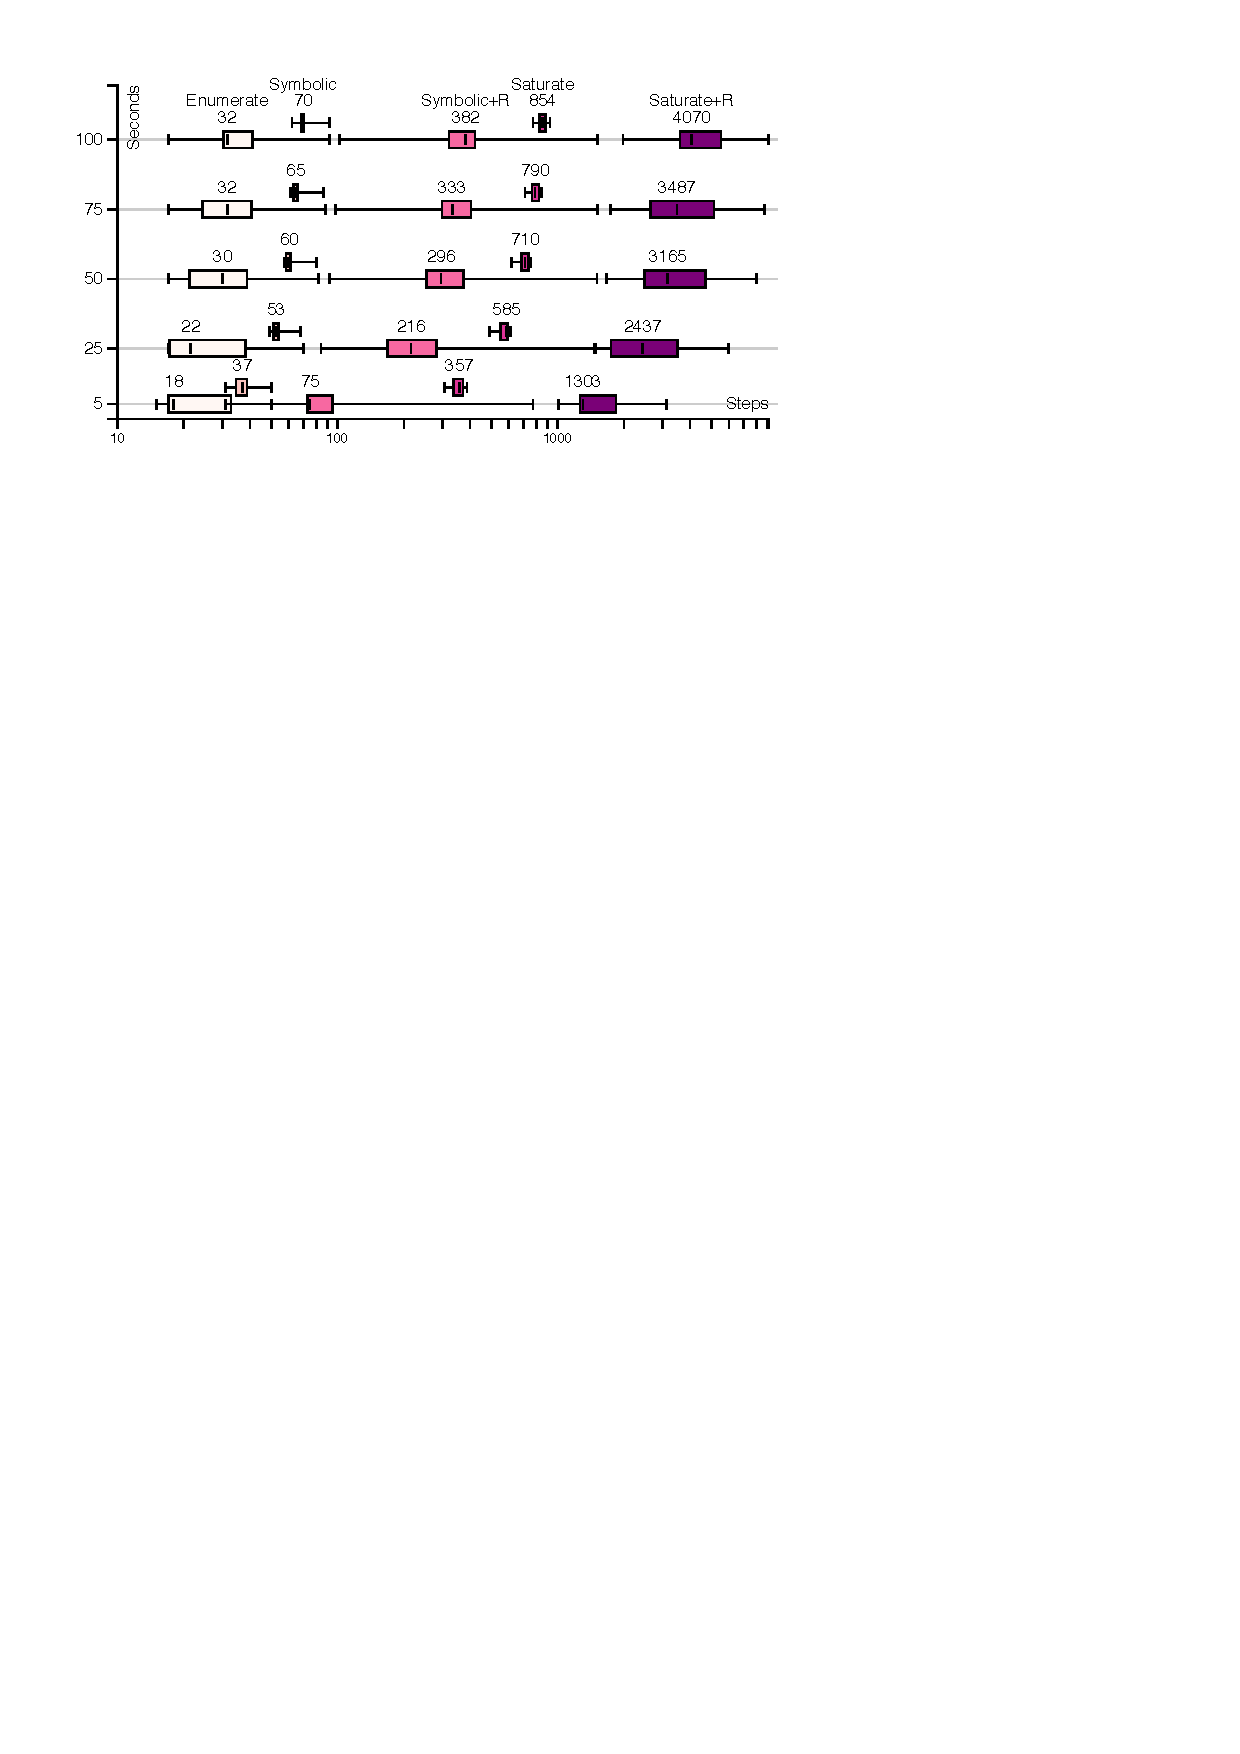
\includegraphics[width=\linewidth]{figures/steps-until-timeout}

  \caption{The number of steps each algorithm is able to process in given time
  limits of $5$s, $25$s, $50$s, $75$s, and $100$s over $10$ histories of Scal’s
  Michael-Scott Queue implementation. Whiskers indicate minimums and maximums,
  numbers indicate medians, and box extents indicate first and third quartiles.
  Steps are plotted to a logarithmic scale.}

  \label{fig:steps}

\end{figure}

Even without match removal, the {\sc saturate} checker achieves a drastic
improvement over {\sc enumerate}, progressing from median $357$ steps in $5$s
to median $854$ steps in $100$s. Most impressively, adding match removal to the
{\sc saturate} checker allows it to process median $1303$ steps in under $5$s.

While the measurements of Figure~\ref{fig:steps} do demonstrate that {\sc
saturate} is more scalable than {\sc enumerate} and {\sc symbolic}, they do not
reveal whether {\sc saturate} scales linearly in the number of steps when match
removal is enabled. This is not visible since the asymptotic complexity of {\sc
saturate} grows polynomially in the \emph{capacity}\footnote{Here
\emph{capacity} means the number of values stored inside the data structure at
a given moment.} of the given concurrent data structures, and the capacities
seen in our pseudo-random executions tend to grow as time goes on.
Figure~\ref{fig:steps:normalized} cancels out the effect of capacity growth by
normalizing data points against the square of the average capacity throughout a
run: for each data point $\tup{s,t,c}$ of $s$ steps in time $t$ with average
capacity $c$, we plot the point $\tup{s,t/c^2}$. Here we clearly see that {\sc
saturate} scales linearly in the number of steps when normalized against
capacity-squared, whereas {\sc enumerate} and {\sc symbolic} continue to scale
poorly despite normalization. The apparent anomaly that {\sc saturate} appears
to scale linearly even with match removal disabled is explained by the fact that
unmatched (add) operations, which could not have been removed in any case, tend
to outnumber matched operations in these recorded histories.

\begin{figure}[t]

  \centering
  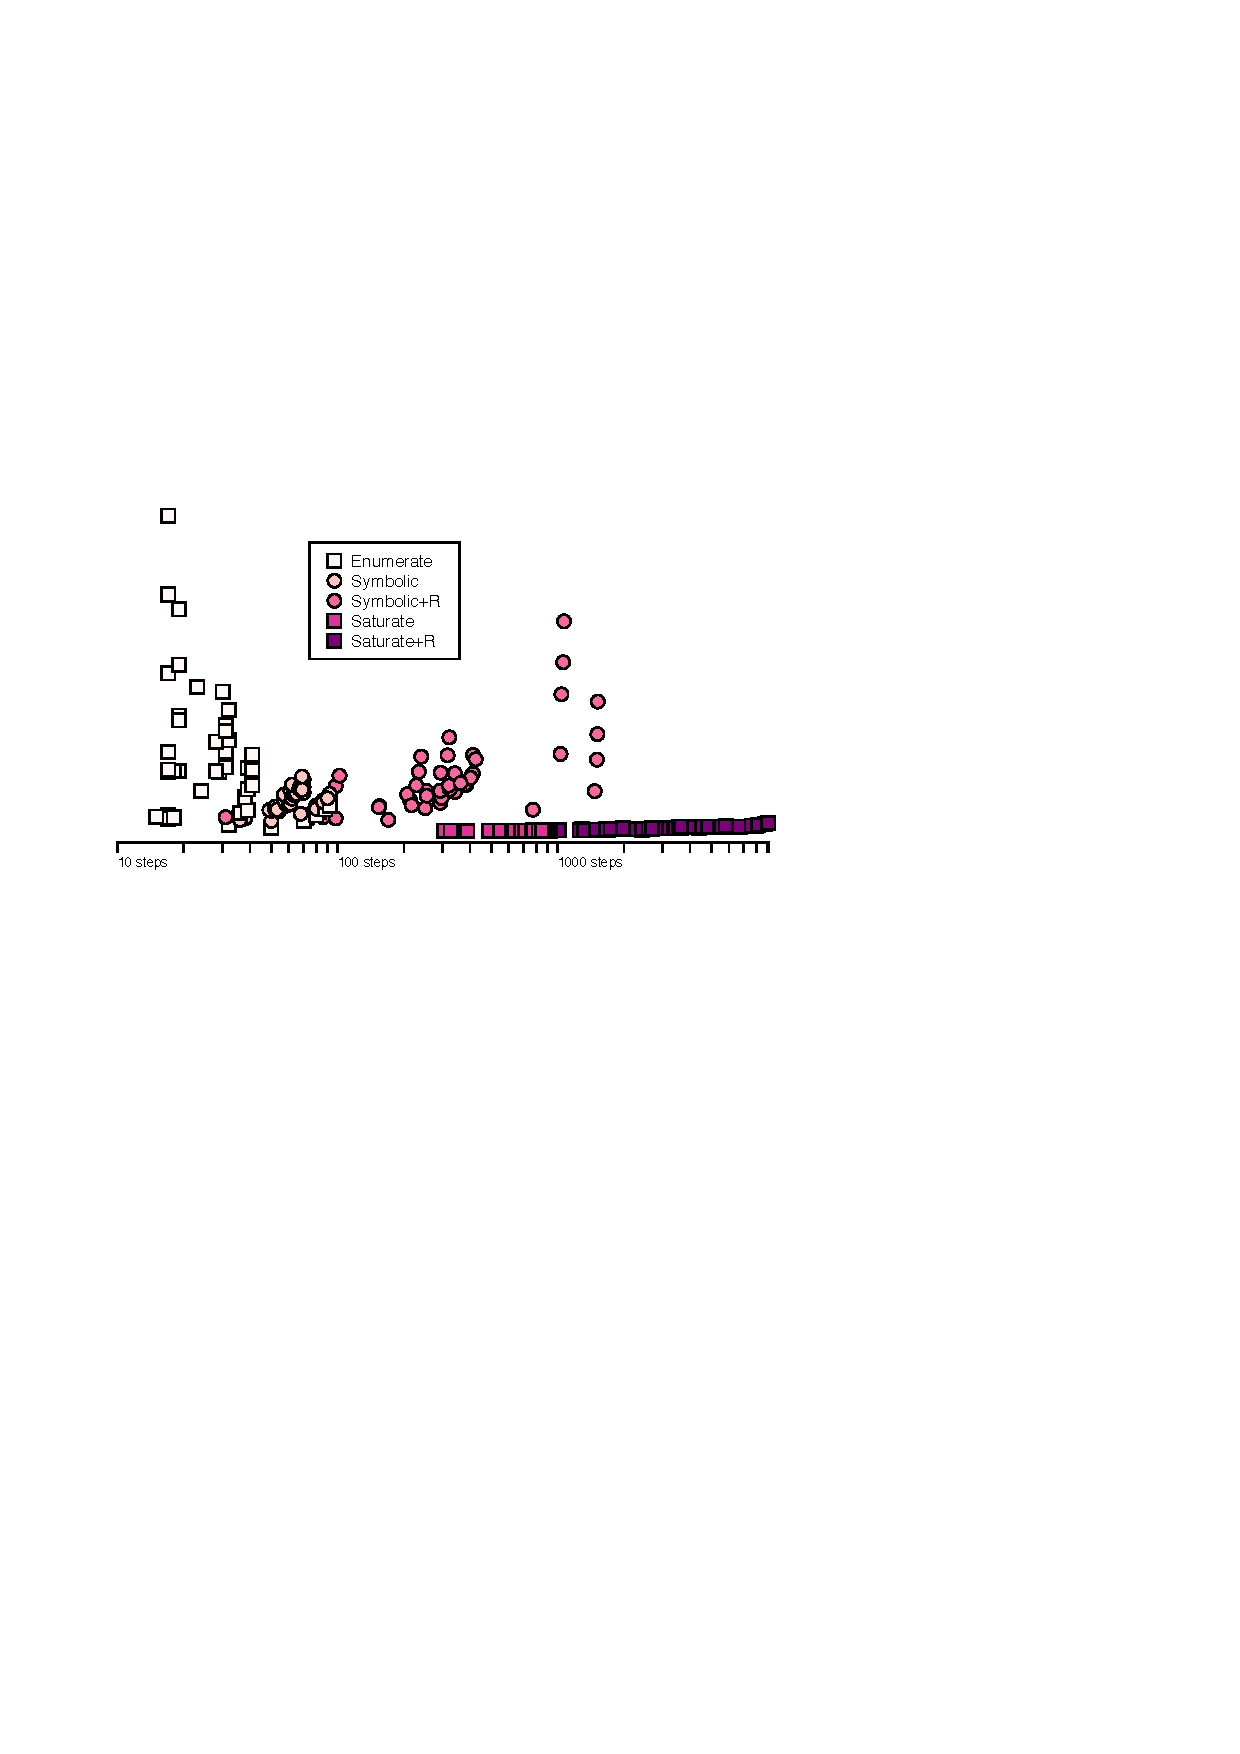
\includegraphics[width=\linewidth]{figures/steps-until-timeout-normalized}

  \caption{The number of steps each algorithm is able to process in time limits
  $5$s, $25$s, $50$s, $75$s, and $100$s normalized by the square of average
  capacity of a given run over 10 histories of Scal’s Michael-Scott Queue
  implementation. Steps are plotted to a logarithmic scale on the x-axis, and
  the y-axis represents normalized time.}

  \label{fig:steps:normalized}

\end{figure}

\subsection{Completeness in Practice}
\label{sec:exp:complete}

Our second experiment measures the amount of violations each algorithm is able
discover across $100$ histories of each of the ten Scal implementations used.
Six of the ten are linearizable, and, correctly, no algorithm reported a
violation therein. The amount of violations detected in the remaining four are
plotted in Figure~\ref{fig:violations}. The {\sc enumerate} algorithm is the
baseline being the most-obviously complete algorithm, and detects all
violations except $1$ for which it exceeds a $10$s timeout. As expected, the
{\sc symbolic} algorithm, also being theoretically complete, also detects all
violations. Validating our hypotheses that the {\sc saturate} algorithm and
match removal are complete in practice, Figure~\ref{fig:violations}
demonstrates that every single violation is also caught by {\sc saturate}, and
enabling removal furthermore does not cause missed violations.

\begin{figure}[t]

  \centering
  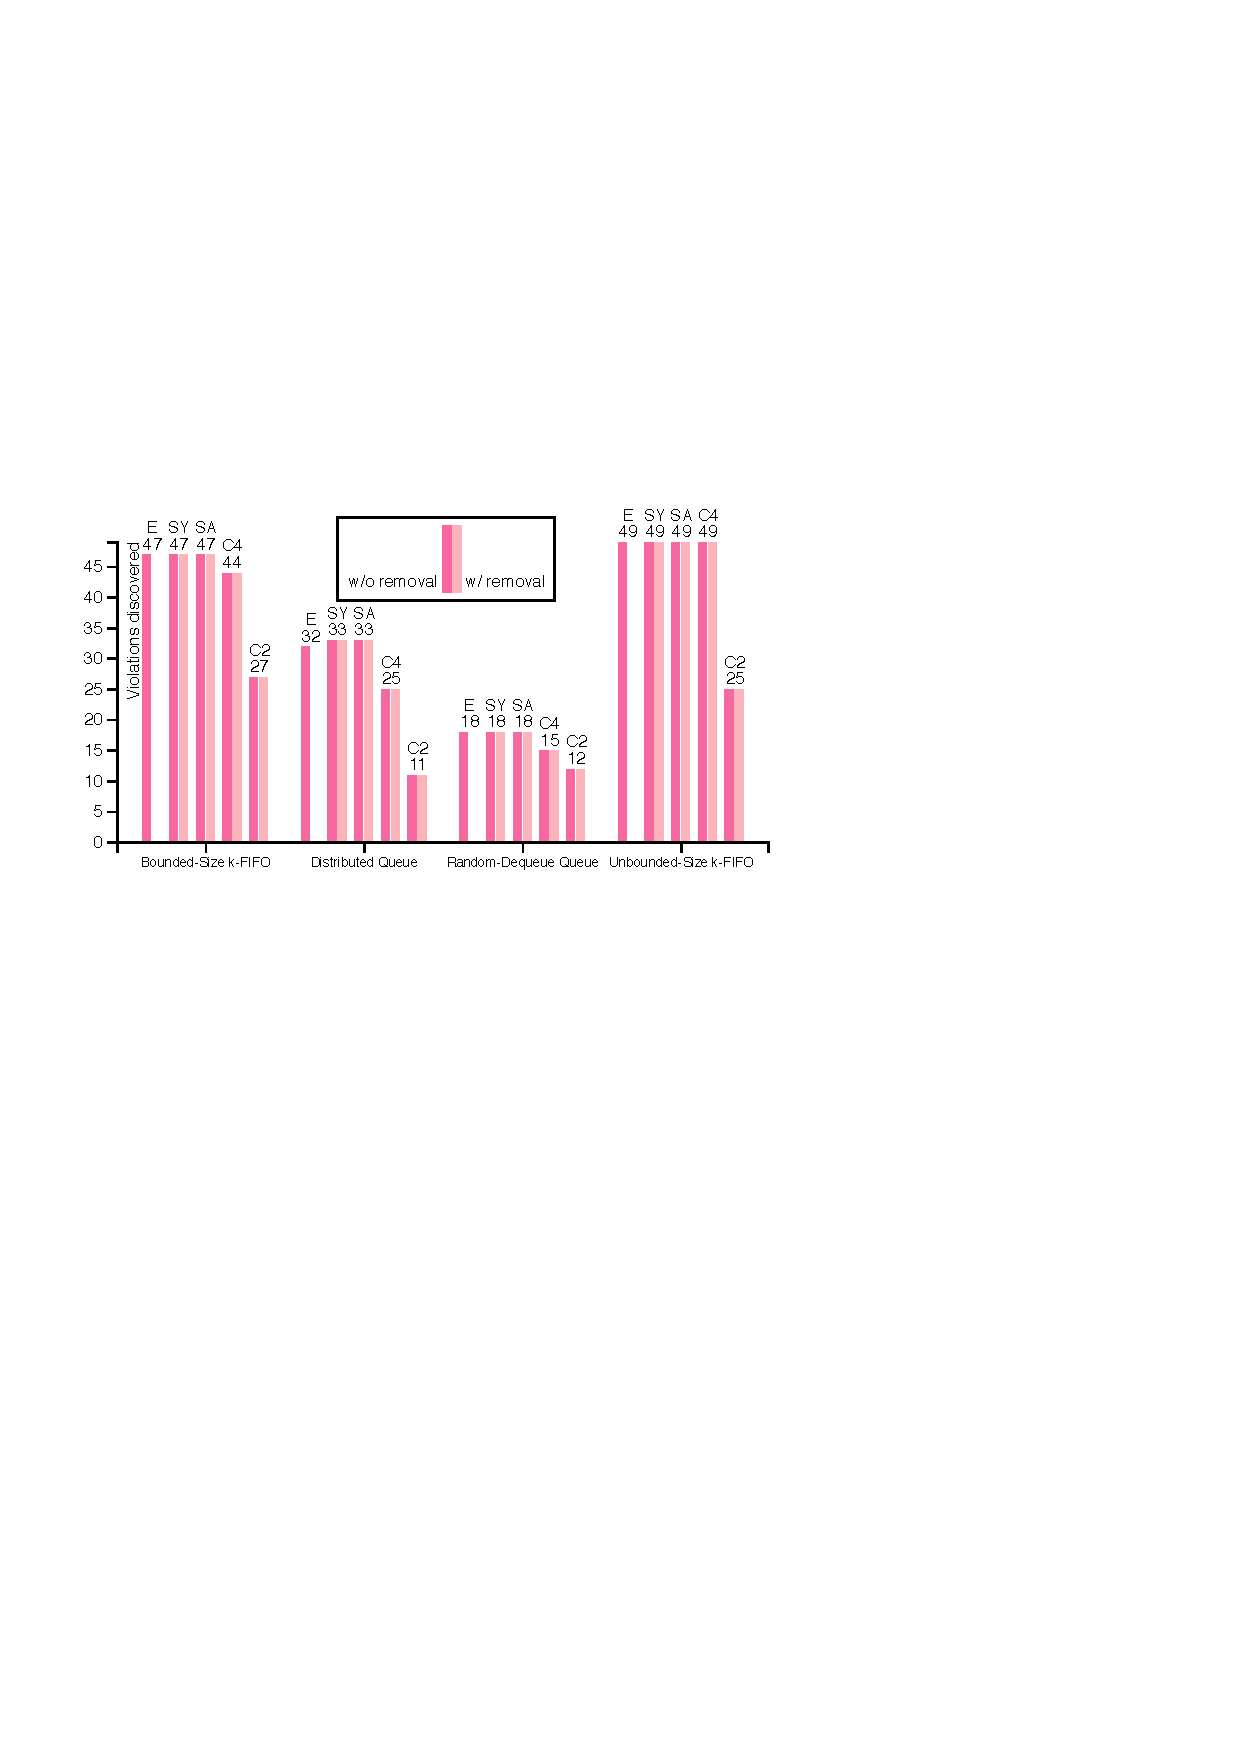
\includegraphics[width=\linewidth]{figures/violations-covered}

  \caption{The number of violations each algorithm is able to detect across
  $100$ histories of each of the four non-linearizable Scal implementations.
  Algorithms are abbreviated: {\sc Enumerate}, {\sc SYmbolic}, {\sc SAturate},
  and {\sc Counting}$(k)$, for $k = 2,4$.}

  \label{fig:violations}

\end{figure}

In order to compare the precision of our algorithms with Bouajjani et
al.~\cite{conf/popl/BouajjaniEEH15}’s parameterized approximation algorithms,
we also plot the number of violations caught using the $k=4$ and $k=2$
approximations. Essentially, their $k$-approximation abstract histories via
weakening by forgetting ordering constraints such that the resulting order is a
$k$-length interval order. As Figure~\ref{fig:violations} demonstrates, while
small values of $k$ can miss many violations, larger values of $k$ can catch
increasingly more, at the expense of additional runtime overhead. To avoid
clutter in Figure~\ref{fig:steps}, we did not plot their runtimes, though we
remark that Bouajjani et al.’s algorithms perform on par with our {\sc
symbolic} algorithm.

Finally, we address the possible sources of incompleteness due to match removal
discussed in Section~\ref{sec:obsolete}. Recall the history $h_1$ and its
extension $h_2$ of Figure~\ref{fig:removal_no_saturation} from
Example~\ref{ex:removal_no_saturation}. Since the {\sc saturate} algorithm does
not speculate on whether the pending rem operation might match the 
add of $2$ or $3$ (or both!), it will not detect the violation in $h_1$ until
the pending rem operation completes. Simply removing the add-rem
match of value $1$ from $h_1$ before the pending rem operation
completes would result in a non-violating history. However, by applying the
stack-theory axioms $\textsc{Theory}(H_\mathrm{st})$ to completed operations
before removing this match, the {\sc saturate} algorithm infers the constraints
\begin{align*}
  \text{add}(2) < \text{add}(1) < (\text{rem} \Rightarrow 1) < (\text{rem} \Rightarrow {\tt empty})
\end{align*}
of which $\text{add}(2) < (\text{rem} \Rightarrow {\tt empty})$ persists after the
match removal. Finally, when the pending \text{rem}-operation does complete,
returning $2$, the {\sc Saturate} algorithm derives a contradiction, since
\begin{align*}
  \text{add}(2) < (\text{rem} \Rightarrow {\tt empty}) < (\text{rem} \Rightarrow 2).
\end{align*}
The incremental nature of the {\sc saturate} algorithm thus avoids the
practically-occurring sources of possible incompleteness due to match removal
of which we are aware.
